\documentclass[conference,letterpaper]{IEEEtran}
\IEEEoverridecommandlockouts
\usepackage[T1]{fontenc}
\usepackage{cite}
\usepackage{amsmath,amssymb}
\usepackage{graphicx}
\usepackage{booktabs}
\usepackage{xurl}
\usepackage[hidelinks]{hyperref}
\newcommand{\blineCom}{91}
\newcommand{\blineRur}{40}
\newcommand{\blineSemi}{98}
\newcommand{\blineUrb}{136}
\newcommand{\btrafoCom}{1}
\newcommand{\btrafoRur}{1}
\newcommand{\btrafoSemi}{1}
\newcommand{\btrafoUrb}{2}
\newcommand{\bvhighCom}{0}
\newcommand{\bvhighRur}{0}
\newcommand{\bvhighSemi}{0}
\newcommand{\bvhighUrb}{0}
\newcommand{\bvlowCom}{11}
\newcommand{\bvlowRur}{53}
\newcommand{\bvlowSemi}{15}
\newcommand{\bvlowUrb}{0}
\newcommand{\corrFirm}{-0.17}
\newcommand{\corrSpread}{0.98}
\newcommand{\corrZth}{0.08}
\newcommand{\depOCom}{14.4}
\newcommand{\depORur}{11.7}
\newcommand{\depOSemi}{12.4}
\newcommand{\depOUrb}{13.1}
\newcommand{\depthPninety}{19}
\newcommand{\depthShareOver}{4.2}
\newcommand{\evOCom}{18.8}
\newcommand{\evORur}{19.0}
\newcommand{\evOSemi}{20.8}
\newcommand{\evOUrb}{18.5}
\newcommand{\eveShare}{38}
\newcommand{\firmPoolMed}{6.1}
\newcommand{\firmmaxCom}{65.1}
\newcommand{\firmmaxRur}{42.8}
\newcommand{\firmmaxSemi}{66.1}
\newcommand{\firmmaxUrb}{22.9}
\newcommand{\firmmedCom}{7.2}
\newcommand{\firmmedRur}{5.6}
\newcommand{\firmmedSemi}{6.2}
\newcommand{\firmmedUrb}{5.8}
\newcommand{\firmminCom}{2.3}
\newcommand{\firmminRur}{1.5}
\newcommand{\firmminSemi}{2.5}
\newcommand{\firmminUrb}{4.6}
\newcommand{\gFCom}{24.9}
\newcommand{\gFRur}{20.9}
\newcommand{\gFSemi}{19.9}
\newcommand{\gFUrb}{21.8}
\newcommand{\gLine}{14.7}
\newcommand{\gOCom}{16.8}
\newcommand{\gORur}{13.3}
\newcommand{\gOSemi}{14.2}
\newcommand{\gOUrb}{15.1}
\newcommand{\gOmaxCom}{23.2}
\newcommand{\gOmaxRur}{23.2}
\newcommand{\gOmaxSemi}{37.8}
\newcommand{\gOmaxUrb}{38.1}
\newcommand{\gOqOCom}{12.9}
\newcommand{\gOqORur}{7.4}
\newcommand{\gOqOSemi}{10.4}
\newcommand{\gOqOUrb}{11.5}
\newcommand{\gOqThCom}{19.3}
\newcommand{\gOqThRur}{21.4}
\newcommand{\gOqThSemi}{15.9}
\newcommand{\gOqThUrb}{22.0}
\newcommand{\gTrafo}{15.2}
\newcommand{\gVlow}{15.7}
\newcommand{\gZFCom}{14.7}
\newcommand{\gZFRur}{11.4}
\newcommand{\gZFSemi}{12.4}
\newcommand{\gZFUrb}{13.2}
\newcommand{\gZTFCom}{13.1}
\newcommand{\gZTFRur}{9.8}
\newcommand{\gZTFSemi}{11.0}
\newcommand{\gZTFUrb}{11.6}
\newcommand{\hOCom}{2945.0}
\newcommand{\hORur}{3072.0}
\newcommand{\hOSemi}{3518.0}
\newcommand{\hOUrb}{3472.4}
\newcommand{\hZTFCom}{1141.0}
\newcommand{\hZTFRur}{1166.6}
\newcommand{\hZTFSemi}{1337.1}
\newcommand{\hZTFUrb}{1167.0}
\newcommand{\hgFZCom}{7.4}
\newcommand{\hgFZRur}{4.6}
\newcommand{\hgFZSemi}{5.8}
\newcommand{\hgFZUrb}{6.0}
\newcommand{\hgOZZCom}{8.5}
\newcommand{\hgOZZRur}{5.4}
\newcommand{\hgOZZSemi}{6.7}
\newcommand{\hgOZZUrb}{7.0}
\newcommand{\hgTZZCom}{9.5}
\newcommand{\hgTZZRur}{6.3}
\newcommand{\hgTZZSemi}{7.6}
\newcommand{\hgTZZUrb}{8.0}
\newcommand{\maxdL}{$10^{-7}$}
\newcommand{\maxdV}{$10^{-10}$}
\newcommand{\nBus}{449}
\newcommand{\nCom}{103}
\newcommand{\nGrids}{4}
\newcommand{\nLine}{365}
\newcommand{\nRur}{94}
\newcommand{\nSemi}{114}
\newcommand{\nTrafo}{5}
\newcommand{\nUrb}{138}
\newcommand{\nVlow}{79}
\newcommand{\poolGadep}{10}
\newcommand{\poolGadepmax}{23}
\newcommand{\poolGaev}{15.0}
\newcommand{\poolGahrs}{1213}
\newcommand{\poolGamax}{30.0}
\newcommand{\poolGamed}{11.5}
\newcommand{\poolGanev}{926}
\newcommand{\poolGaqa}{8.1}
\newcommand{\poolGaqc}{15.7}
\newcommand{\poolGbmax}{33.8}
\newcommand{\poolGbmed}{13.0}
\newcommand{\poolGbqa}{9.4}
\newcommand{\poolGbqc}{17.7}
\newcommand{\poolGcdep}{13}
\newcommand{\poolGcdepmax}{28}
\newcommand{\poolGcev}{19.0}
\newcommand{\poolGchrs}{3350}
\newcommand{\poolGcmax}{38.1}
\newcommand{\poolGcmed}{15.0}
\newcommand{\poolGcmedev}{0.8}
\newcommand{\poolGcmedevmin}{45}
\newcommand{\poolGcnev}{1263}
\newcommand{\poolGcqa}{10.9}
\newcommand{\poolGcqc}{19.9}
\newcommand{\poolGcsingle}{34}
\newcommand{\poolGdmax}{52.6}
\newcommand{\poolGdmed}{21.7}
\newcommand{\poolGdqa}{16.5}
\newcommand{\poolGdqc}{29.1}
\newcommand{\poolHFZen}{0.007}
\newcommand{\poolHFZmed}{5.9}
\newcommand{\poolHOZZen}{0.013}
\newcommand{\poolHOZZmed}{6.8}
\newcommand{\poolHOZen}{0.001}
\newcommand{\poolHOZmed}{3.9}
\newcommand{\poolHOen}{0.000}
\newcommand{\poolHOmed}{1.4}
\newcommand{\poolHTZZen}{0.029}
\newcommand{\poolHTZZmed}{7.8}
\newcommand{\snapLmaxCom}{10.2}
\newcommand{\snapLmaxRur}{18.0}
\newcommand{\snapLmaxSemi}{49.9}
\newcommand{\snapLmaxUrb}{15.8}
\newcommand{\snapOverMax}{12.5}
\newcommand{\snapOverShare}{42}
\newcommand{\snapmaxCom}{8.1}
\newcommand{\snapmaxRur}{12.5}
\newcommand{\snapmaxSemi}{1.9}
\newcommand{\snapmaxUrb}{1.4}
\newcommand{\snapmedCom}{3.0}
\newcommand{\snapmedRur}{0.7}
\newcommand{\snapmedSemi}{0.7}
\newcommand{\snapmedUrb}{0.1}
\newcommand{\spreadMed}{16.0}
\newcommand{\winShare}{43}

\newcommand{\sensBasefirm}{6.1}
\newcommand{\sensBasegO}{15.0}
\newcommand{\sensBasegZTF}{11.5}
\newcommand{\sensBasegl}{14.7}
\newcommand{\sensBasegv}{15.7}
\newcommand{\sensBasehOZZ}{6.8}
\newcommand{\sensBasehrsO}{3350.2}
\newcommand{\sensBasenbus}{449}
\newcommand{\sensBasenl}{365}
\newcommand{\sensBasent}{5}
\newcommand{\sensBasenv}{79}
\newcommand{\sensFixfirm}{5.9}
\newcommand{\sensFixgO}{16.7}
\newcommand{\sensFixgZTF}{13.2}
\newcommand{\sensFixgl}{15.3}
\newcommand{\sensFixgv}{28.5}
\newcommand{\sensFixhOZZ}{8.2}
\newcommand{\sensFixhrsO}{3189.8}
\newcommand{\sensFixnbus}{449}
\newcommand{\sensFixnl}{341}
\newcommand{\sensFixnt}{2}
\newcommand{\sensFixnv}{106}
\newcommand{\sensHRangeHi}{30}
\newcommand{\sensHRangeLo}{6}
\newcommand{\sensNmofirm}{2.9}
\newcommand{\sensNmogO}{50.3}
\newcommand{\sensNmogZTF}{38.7}
\newcommand{\sensNmogl}{45.2}
\newcommand{\sensNmogv}{55.0}
\newcommand{\sensNmohOZZ}{29.4}
\newcommand{\sensNmohrsO}{1535.5}
\newcommand{\sensNmonbus}{449}
\newcommand{\sensNmonl}{203}
\newcommand{\sensNmont}{5}
\newcommand{\sensNmonv}{241}
\newcommand{\sensNmowfirm}{3.6}
\newcommand{\sensNmowgO}{38.8}
\newcommand{\sensNmowgZTF}{29.2}
\newcommand{\sensNmowgl}{50.6}
\newcommand{\sensNmowgv}{22.5}
\newcommand{\sensNmowhOZZ}{20.2}
\newcommand{\sensNmowhrsO}{1780.8}
\newcommand{\sensNmownbus}{449}
\newcommand{\sensNmownl}{328}
\newcommand{\sensNmownt}{5}
\newcommand{\sensNmownv}{116}
\newcommand{\sensRangeHi}{51}
\newcommand{\sensRangeLo}{14}
\newcommand{\sensStwofirm}{5.9}
\newcommand{\sensStwogO}{18.8}
\newcommand{\sensStwogZTF}{14.1}
\newcommand{\sensStwogl}{18.1}
\newcommand{\sensStwogv}{23.4}
\newcommand{\sensStwohOZZ}{8.1}
\newcommand{\sensStwohrsO}{2492.8}
\newcommand{\sensStwonbus}{460}
\newcommand{\sensStwonl}{373}
\newcommand{\sensStwont}{5}
\newcommand{\sensStwonv}{82}
\newcommand{\shpRowFirm}{6.24}
\newcommand{\shpRowGone}{17.4}
\newcommand{\shpRowHrs}{1727}

\newcommand{\shpDCFoZatOFfe}{$-$18.6}
\newcommand{\shpDCFoZatOFfp}{1.7}
\newcommand{\shpDCFoZatOFgO}{17.4}
\newcommand{\shpDCFoZatOFhrs}{1727}
\newcommand{\shpDCFoZatThfe}{$-$9.0}
\newcommand{\shpDCFoZatThfp}{13.7}
\newcommand{\shpDCFoZatThgO}{9.1}
\newcommand{\shpDCFoZatThhrs}{2185}
\newcommand{\shpDCTZatOFfe}{$-$8.8}
\newcommand{\shpDCTZatOFfp}{1.3}
\newcommand{\shpDCTZatOFgO}{16.7}
\newcommand{\shpDCTZatOFhrs}{2170}
\newcommand{\shpDCTZatONfe}{$-$9.5}
\newcommand{\shpDCTZatONfp}{0.5}
\newcommand{\shpDCTZatONgO}{17.4}
\newcommand{\shpDCTZatONhrs}{2217}
\newcommand{\shpDCTZatThfe}{$-$1.2}
\newcommand{\shpDCTZatThfp}{9.8}
\newcommand{\shpDCTZatThgO}{10.5}
\newcommand{\shpDCTZatThhrs}{3163}
\newcommand{\shpFlatfe}{0.0}
\newcommand{\shpFlatfp}{0.0}
\newcommand{\shpFlatgO}{15.0}
\newcommand{\shpFlathrs}{3350}
\newcommand{\shpTrack}{15.9}

\newcommand{\robDayaddMW}{0.13}
\newcommand{\robDaygain}{2.2}
\newcommand{\robDayhrs}{2918}
\newcommand{\robDaym}{9}
\newcommand{\robDayqa}{1.3}
\newcommand{\robDayqc}{2.9}
\newcommand{\robFifteenaddMW}{0.36}
\newcommand{\robFifteengain}{6.1}
\newcommand{\robFifteenhrs}{3254}
\newcommand{\robFifteenm}{7}
\newcommand{\robFifteenqa}{4.7}
\newcommand{\robFifteenqc}{7.6}
\newcommand{\robPerfaddMW}{0.82}
\newcommand{\robPerfgain}{15.0}
\newcommand{\robPerfhrs}{3352}
\newcommand{\robPerfm}{0}
\newcommand{\robPerfqa}{10.9}
\newcommand{\robPerfqc}{19.9}

\newcommand{\audBoundaryM}{15.8}
\newcommand{\audMonoK}{42}
\newcommand{\audValMax}{3.4}
\newcommand{\audValMed}{0.4}
\newcommand{\audValN}{295}
\newcommand{\audValOvt}{55}
\newcommand{\gonepctint}{6.7}
\newcommand{\nOnePPN}{60}
\newcommand{\nOnePPOK}{60}

\newcommand{\oosDaygain}{2.7}
\newcommand{\oosDayviol}{52}
\newcommand{\oosFifteengain}{6.7}
\newcommand{\oosFifteenviol}{35}
\newcommand{\oosHDayviol}{49}
\newcommand{\oosHFifteenviol}{33}

\newcommand{\fsCases}{2103}
\newcommand{\fsSteps}{4.1}

\newcommand{\battOMWh}{116.4}
\newcommand{\battOh}{128}
\newcommand{\battOMW}{0.83}
\newcommand{\battOadd}{0.83}
\newcommand{\battQMWh}{4.8}
\newcommand{\battQh}{7}
\newcommand{\battQMW}{0.62}
\newcommand{\battQadd}{0.62}

\newcommand{\spZth}{0.01}
\newcommand{\spFirm}{$-$0.18}
\newcommand{\depthHundred}{6}

\newcommand{\pfN}{100}
\newcommand{\pfFirm}{5.7}
\newcommand{\pfGainA}{15.1}
\newcommand{\pfGainB}{14.6}

\newcommand{\cpLo}{185}
\newcommand{\cpHi}{258}

\newcommand{\fsxCases}{2103}

\newcommand{\fcBestDagain}{3.2}
\newcommand{\fcBestDaviol}{53}
\newcommand{\fcBestFifteengain}{6.7}
\newcommand{\fcBestFifteenviol}{35}
\newcommand{\fcExcHi}{1.6}
\newcommand{\fcExcLo}{1.0}
\newcommand{\fcMapeHi}{1.7}
\newcommand{\fcMapeLo}{0.6}
\newcommand{\fcNLDagain}{3.2}
\newcommand{\fcNLDam}{9}
\newcommand{\fcNLDamape}{1.4}
\newcommand{\fcNLDaviol}{53}
\newcommand{\fcNLFifteengain}{5.7}
\newcommand{\fcNLFifteenm}{7}
\newcommand{\fcNLFifteenmape}{0.7}
\newcommand{\fcNLFifteenviol}{40}
\newcommand{\fcPDagain}{2.7}
\newcommand{\fcPDam}{8}
\newcommand{\fcPDamape}{1.7}
\newcommand{\fcPDaviol}{52}
\newcommand{\fcPFifteengain}{6.7}
\newcommand{\fcPFifteenm}{7}
\newcommand{\fcPFifteenmape}{0.6}
\newcommand{\fcPFifteenviol}{35}
\newcommand{\fcRangeDagainHi}{3.2}
\newcommand{\fcRangeDagainLo}{2.3}
\newcommand{\fcRangeDaviolHi}{53}
\newcommand{\fcRangeDaviolLo}{48}
\newcommand{\fcRangeFifteengainHi}{6.7}
\newcommand{\fcRangeFifteengainLo}{5.7}
\newcommand{\fcRangeFifteenviolHi}{41}
\newcommand{\fcRangeFifteenviolLo}{35}
\newcommand{\fcSAFifteengain}{5.7}
\newcommand{\fcSAFifteenm}{7}
\newcommand{\fcSAFifteenmape}{0.7}
\newcommand{\fcSAFifteenviol}{41}
\newcommand{\fcSNDtgain}{2.3}
\newcommand{\fcSNDtm}{8}
\newcommand{\fcSNDtmape}{1.6}
\newcommand{\fcSNDtviol}{48}
\newcommand{\fcSNWgain}{2.3}
\newcommand{\fcSNWm}{9}
\newcommand{\fcSNWmape}{1.7}
\newcommand{\fcSNWviol}{49}
\newcommand{\fcVintHi}{4}
\newcommand{\fcVintLo}{1}

\newcommand{\ciAddHi}{0.96}
\newcommand{\ciAddLo}{0.69}
\newcommand{\ciFirmHi}{6.61}
\newcommand{\ciFirmLo}{5.85}
\newcommand{\ciGoneHi}{16.1}
\newcommand{\ciGoneLo}{12.9}
\newcommand{\ciGqHi}{12.7}
\newcommand{\ciGqLo}{9.6}
\newcommand{\ciHHi}{7.8}
\newcommand{\ciHLo}{5.4}
\newcommand{\ciHrsHi}{3537}
\newcommand{\ciHrsLo}{3004}
\newcommand{\depOne}{13}
\newcommand{\hrsOneShare}{38}
\newcommand{\logoHi}{15.3}
\newcommand{\logoLo}{14.7}
\newcommand{\nClusters}{17}

\newcommand{\ctAadd}{0.62}
\newcommand{\ctAdep}{10}
\newcommand{\ctAen}{0.25}
\newcommand{\ctAfirm}{6.13}
\newcommand{\ctAgain}{11.5}
\newcommand{\ctAhrs}{1213}
\newcommand{\ctAmed}{30}
\newcommand{\ctAmx}{15.0}
\newcommand{\ctAnev}{926}
\newcommand{\ctBadd}{0.82}
\newcommand{\ctBdep}{13}
\newcommand{\ctBen}{1.00}
\newcommand{\ctBfirm}{6.13}
\newcommand{\ctBgain}{15.0}
\newcommand{\ctBhrs}{3350}
\newcommand{\ctBmed}{45}
\newcommand{\ctBmx}{19.0}
\newcommand{\ctBnev}{1263}
\newcommand{\ctHadd}{0.34}
\newcommand{\ctHdep}{6}
\newcommand{\ctHen}{0.01}
\newcommand{\ctHfirm}{6.13}
\newcommand{\ctHgain}{6.8}
\newcommand{\ctHhrs}{100}
\newcommand{\ctHmed}{15}
\newcommand{\ctHmx}{3.3}
\newcommand{\ctHnev}{224}
\newcommand{\ctNadd}{1.32}
\newcommand{\ctNdep}{33}
\newcommand{\ctNen}{1.00}
\newcommand{\ctNfirm}{2.88}
\newcommand{\ctNgain}{50.3}
\newcommand{\ctNhrs}{1536}
\newcommand{\ctNmed}{30}
\newcommand{\ctNmx}{15.8}
\newcommand{\ctNnev}{1060}
\newcommand{\gEightyFive}{6.6}

\newcommand{\nmoN}{444}
\newcommand{\nmoUnr}{20}
\newcommand{\nmoMulti}{137}
\newcommand{\nmoSpread}{64}

\newcommand{\todEveen}{0.1}
\newcommand{\todEvegain}{0.2}
\newcommand{\todEvehrs}{2196}
\newcommand{\todEvevOT}{42}
\newcommand{\todEvevTO}{57}
\newcommand{\todEveviol}{50}
\newcommand{\todWinEveen}{0.0}
\newcommand{\todWinEvegain}{0.1}
\newcommand{\todWinEvehrs}{726}
\newcommand{\todWinEvevOT}{45}
\newcommand{\todWinEvevTO}{55}
\newcommand{\todWinEveviol}{50}
\newcommand{\todWinen}{1.0}
\newcommand{\todWingain}{3.1}
\newcommand{\todWinhrs}{2904}
\newcommand{\todWinvOT}{30}
\newcommand{\todWinvTO}{70}
\newcommand{\todWinviol}{50}

\newcommand{\depCap}{25}
\newcommand{\depMaxGain}{33}
\newcommand{\depNOgain}{33.3}
\newcommand{\depNOshare}{79}
\newcommand{\depNZgain}{15.0}
\newcommand{\depNZshare}{4}

\newcommand{\corCorMW}{6.90}
\newcommand{\corDepth}{55}
\newcommand{\corDepthQa}{45}
\newcommand{\corDepthQc}{73}
\newcommand{\corExtraMW}{2.15}
\newcommand{\corPreMW}{4.33}


\begin{document}

\title{Hosting Capacity Gains and Curtailment Burden of Flexible Connections for Large Medium-Voltage Loads}

\author{\IEEEauthorblockN{Heng Yao (Jacob) Wang\thanks{The author is an incoming undergraduate student at The Wharton School, University of Pennsylvania, Philadelphia, PA, USA.}}
\IEEEauthorblockA{Independent Researcher, Singapore\\
jwjw88073@gmail.com}}

\maketitle

\begin{abstract}
Large new loads at medium voltage (MV), such as data centers, charging hubs, and electrified industry, often wait for network reinforcement before they can connect. Flexible connections that allow curtailment are a proposed remedy, but their value at the connection point is rarely quantified. For all \nBus~MV buses of the four SimBench MV grids, this paper computes the largest flat load that a single new connection can add in each 15-min interval of a year under AC voltage and thermal limits, and compares firm, snapshot, energy-budget, and hour-budget hosting capacity. With all lines in service, curtailing 1\% of annual energy raises hosting capacity by a median of \poolGcmed\% but requires curtailment in about \poolGchrs~h/yr. A fixed seasonal curtailment schedule with a similar energy loss gains only \todWingain\%, and forecasts from past data keep less than half of the gain while still violating limits out of sample. Where the network is planned for N-1 line outages with preventive curtailment, the gain rises to \sensNmogO\%. Flexible connection terms should therefore specify hours, events, and response requirements, not energy alone.
\end{abstract}

\begin{IEEEkeywords}
Demand response, distribution networks, flexible connection, hosting capacity, power system planning
\end{IEEEkeywords}

\section{Introduction}
U.S. data centers used about 4.4\% of national electricity in 2023, with projections of 6.7--12\% by 2028 \cite{lbnl}, and global data-center consumption is expected to more than double by 2030 \cite{iea}. Loads of a few to tens of MW, including smaller data centers, charging hubs, and electrified industry, connect at MV, where the network operator must confirm that voltage and thermal limits hold under all expected conditions; otherwise the load waits for reinforcement. A study of 22 U.S. balancing authorities estimated that 76--126~GW of new large load could be integrated if it accepted curtailment of 0.25--1\% of its maximum potential annual energy (about 85~h/yr at 0.25\%) \cite{duke,utilitydive2025}; it does not model distribution networks.

Non-firm connections are established for distributed generation (DG). Active network management curtails generators when measured flows approach limits \cite{currie2007}, principles of access decide who is curtailed first \cite{kane2014}, and curtailment-based HC has been quantified \cite{anaya2015,kulmala2017}. Operating envelopes compute, ahead of each interval, the import and export limits that keep a network within its limits \cite{petrou2021,liu2022} and can raise electric-vehicle (EV) HC \cite{fani2024}; firm and non-firm HC for DG and EVs are compared in \cite{zakaria2025}, and a security-aware dynamic HC for DG includes N-1 contingencies and their probabilities \cite{herding2024}. Flexible agreements are proposed to manage connection queues \cite{desanti2025} and are being extended to loads \cite{doe2024}, including hour-limited transmission products with day-ahead notice \cite{tennet_tdtr}; on data-center demand response, see \cite{wierman2014,colangelo2025}.

Hosting capacity (HC) is the amount of new production or consumption that can be connected before a performance limit is reached \cite{bollen2017}. Most HC studies address DG \cite{ismael2019,benzerga2025,mulenga2020} or EVs \cite{umoh2023}, and time-series analysis can give higher HC than a worst-case snapshot \cite{jain2019}. For flexible loads, Gu \emph{et al.} \cite{gu2026hicss} capped the number of curtailed intervals, showed that the optimal capacity is an order statistic of the per-interval headroom, and extended this to partially measured grids \cite{gu2026eenergy}; Sarker and Dahlin \cite{sarker2026} added depth and tail-risk limits. Both use a copperplate model or one bus of the IEEE 123-bus feeder with a linearized power flow without line thermal limits. Relative to \cite{gu2026hicss,sarker2026}, this paper contributes:
\begin{enumerate}
\item An AC assessment with voltage, line, and transformer limits of every MV bus (\nBus) of the four SimBench grids \cite{simbench} over a full year at 15-min resolution, with intact lines and with N-1 line outages and restoration switching.
\item A comparison, from one headroom series per bus, of firm, snapshot, energy-budget, and hour-budget HC, with the curtailment hours, events, and depth each implies, translated into contract parameters.
\item Out-of-sample tests of imperfect foresight with persistence, seasonal-naive, and net-load-based forecasts, a fixed-schedule baseline, and other sensitivity tests.
\end{enumerate}
The new load is a generic flat load; no data-center operating profile is modeled.

\section{Methodology}
\subsection{Headroom Series}
Consider a balanced MV network with bus set $\mathcal N$. In interval $t\in\mathcal T$ the existing loads, DG, and storage inject complex power $\mathbf s_t$. One new load at bus $k$, with no other new connections, draws $P(1+j\tan\varphi)$ at constant power factor $\cos\varphi$. Let $\mathbf V(P,t)$ be the AC power-flow solution. The limits are
\begin{align}
\underline v_i \le |V_i| \le \overline v_i,\quad |I_\ell|\le I_\ell^{\max},\quad |I_m|\le I_m^{\max},
\end{align}
for all buses $i$, lines $\ell$, and transformers $m$. Write each limit $e$ (lower and upper voltage limits separately) as a margin $m_e(P,t)\ge 0$, scaled per limit type (voltage in units of 0.05~p.u., current as a fraction of rating). Some intervals violate a limit before any load is added; in our data only overvoltages from DG, which SimBench models at unity power factor without voltage control. The new load must create no new violation and worsen no existing one:
\begin{equation}
\bar P_k(t)=\max\{P\ge 0:\ m_e(P,t)\ge\min[0,m_e(0,t)]\ \forall e\},\label{eq:head}
\end{equation}
with a tolerance of $10^{-7}$. Without pre-existing violations, \eqref{eq:head} reduces to the limits in (1).

\subsection{Hosting-Capacity Definitions}
The \emph{firm} HC is $H_k^{\mathrm{firm}}=\min_{t}\bar P_k(t)$. The \emph{snapshot} HC $\bar P_k(t^\ast)$ evaluates one interval $t^\ast$, here the interval of highest grid-wide net active load (load minus DG). A flexible load of nameplate $P$ is curtailed to $\bar P_k(t)$ whenever $P>\bar P_k(t)$. Its curtailed energy is $E_k(P)=\Delta t\sum_t[P-\bar P_k(t)]^+$, and the \emph{energy-budget} HC for a fraction $\alpha$ of its maximum potential annual energy (as in \cite{duke}) is
\begin{equation}
H_k(\alpha)=\max\{P\le \max_t\bar P_k(t):\ E_k(P)\le \alpha\,P\,|\mathcal T|\,\Delta t\}.\label{eq:flex}
\end{equation}
Because $E_k(P)/P$ is non-decreasing in $P$, \eqref{eq:flex} is solved by bisection. The \emph{hour-budget} HC $H_k^{h}(N)$ allows curtailment of any depth in at most $N$ hours per year; as in \cite{gu2026hicss}, it is the $(N/\Delta t+1)$-th smallest value of $\bar P_k(t)$. With $\Delta t=0.25$~h and the leap year 2016, $|\mathcal T|=35\,136$ intervals (8784~h); an event is a run of consecutive curtailed intervals. Gains are $H/H_k^{\mathrm{firm}}-1$.

Curtailment above assumes perfect foresight. With imperfect foresight the load draws $L(t)=\min\{P,(1-\mu)\hat P_k(t)\}$, where $\hat P_k(t)$ is a forecast of $\bar P_k(t)$ from past data only and $\mu$ is a safety margin. $P$ and $\mu\in\{0,0.01,\dots,0.30\}$ are chosen jointly on training weeks to maximize $P$ subject to $L(t)\le\bar P_k(t)$ in every training interval and $\Delta t\sum_t[P-L(t)]\le\alpha P|\mathcal T_{\mathrm{train}}|\Delta t$ (margin-induced curtailment counts against the budget), and are then applied unchanged to the test weeks (alternating weeks, both directions). With a 15-min horizon (data up to $t-1$) the forecasts are persistence, $\bar P_k(t-1)$; seasonally adjusted persistence, $\bar P_k(t-1)+B_k(t)-B_k(t-1)$, with $B_k$ the mean headroom at the same time on the last four days of the same type (weekday, Saturday, Sunday); and a net-load forecast, the headroom from \eqref{eq:head} for injections $\mathbf s_{t-1}+\bar{\mathbf s}_t-\bar{\mathbf s}_{t-1}$, with $\bar{\mathbf s}$ the analogous mean of the injections. Day-ahead forecasts (data up to the previous midnight) are $\bar P_k(t-96)$, $\bar P_k(t-672)$, the latest same-type day, and the headroom for $\bar{\mathbf s}_t$.

\subsection{Vectorized Power Flow and Headroom Search}
We solve all intervals at once. Let $\mathcal R$ be the slack buses with voltages $\mathbf V_{\mathcal R}$, $\mathcal N'$ the other buses, and $\mathbf Y$ the bus admittance matrix. The Z-bus fixed-point iteration
\begin{equation}
\mathbf V^{(\nu+1)}_{\mathcal N'}=\mathbf Z\big(\overline{\mathbf S_{\mathcal N'}\oslash \mathbf V^{(\nu)}_{\mathcal N'}}-\mathbf Y_{\mathcal N'\mathcal R}\mathbf V_{\mathcal R}\big),\ \ \mathbf Z=\mathbf Y_{\mathcal N'\mathcal N'}^{-1},\label{eq:zbus}
\end{equation}
is applied to a matrix whose 35\,136 columns are the intervals \cite{salazar2024tensor}. Here $\mathbf S$ is the net injection including the new load, the overline denotes conjugation, and $\oslash$ element-wise division. Iterations stop at a voltage change below $10^{-9}$~p.u. or after 60 iterations; columns whose last change exceeds $10^{-6}$~p.u. are treated as infeasible. Convergence conditions are given in \cite{bolognani2016,wang2018,bazrafshan2018}; we did not check them, but no non-converged case occurred. $\mathbf Y$, branch matrices, and limits come from pandapower \cite{pandapower}. With \emph{fixed taps}, the transformers keep their SimBench tap positions and the high-voltage (HV) bus is the slack at 1.025~p.u. With an \emph{ideal on-load tap changer (OLTC)}, the transformers are removed and each MV busbar is a slack bus at the 1.025~p.u. set point; transformer current equals the busbar injection, shared equally where two units feed one busbar. This omits transformer impedance, losses, and the tap range. $\bar P_k(t)$ is found for all $t$ at once by a bracketed Illinois search on the smallest margin in \eqref{eq:head}, stopping when a feasible and an infeasible bracket are 5~kW apart and reporting the feasible one. This assumes that the feasible set is $[0,\bar P_k(t)]$, which is not guaranteed for AC power flow and is tested below.

\subsection{Verification}\label{sec:val}
Against pandapower's Newton-Raphson solution, voltage differences were below \maxdV~p.u. and loading differences below \maxdL~percentage points. An independent pandapower bisection on \audValN~stratified cases (including \audValOvt~intervals with pre-existing overvoltage) matched the headroom within \audValMax~kW (median \audValMed~kW), with the same limiting class in every case. For all \audBoundaryM~million bus-intervals, the headroom was feasible under \eqref{eq:head} and infeasible 6~kW above it. The search applies \eqref{eq:head} per limit class; because only overvoltages pre-existed and no bus's overvoltage grew, this equals the element-wise rule. On monotonicity, 5-kW scans from 0 to $1.3\bar P_k(t)$ at \fsCases~bus-intervals (including each bus's worst interval, the largest reverse power flow, and pre-existing overvoltages; \fsSteps~million power flows), 20-kW scans to $3\bar P_k(t)$, and 60 pandapower scans never found feasibility regained above the first violation; this supports, but does not prove, monotonicity. For N-1 (Section~\ref{sec:sens}), \nOnePPOK~of \nOnePPN~random outage-limited cases rebuilt in pandapower passed the same boundary test.

\section{Case Study}
We use the four MV grids of SimBench \cite{simbench} (scenario 0, switching variant) with their 2016 synthetic load and DG profiles at 15-min resolution (Table~\ref{tab:grids}). Every MV bus is a candidate, \nBus~in total. Voltage limits are SimBench's per-bus planning bands, 0.965--1.055~p.u. at MV. SimBench specifies automatic HV/MV taps with a 1.025~p.u. set point, so the base case uses the ideal OLTC. In the base case lines are limited to 100\% of rated current with all lines in service (N-0), and transformers to the SimBench maximum loading (50\% in the urban grid, so one transformer can carry the load if the other fails; 100\% otherwise). The N-1 case is described in Section~\ref{sec:sens}. The new load is flat at nameplate with $\cos\varphi=0.95$ lagging. One full-year power flow takes about 1~s and the headroom search 10--35~s per bus on a two-core 2.8~GHz Xeon. Code, results, and a script that regenerates every table and figure are at \url{https://github.com/jacobwanghy/flexible-load-hc}.

\begin{table}[t]
\centering
\caption{SimBench MV Grids (Scenario 0)}
\label{tab:grids}
\setlength{\tabcolsep}{2.8pt}
\begin{tabular}{lcccccc}
\toprule
Grid & $V_n$ & Buses & HV/MV & Peak & Peak net & DG \\
 & (kV) & (MV) & (MVA) & load (MW) & load (MW) & (MW) \\
\midrule
Rural & 20 & 94 & $2\times25$ & 7.5 & 6.3 & 25.6 \\
Semi-urban & 20 & 114 & $2\times40$ & 13.4 & 12.1 & 23.8 \\
Urban & 10 & 138 & $2\times63$ & 21.0 & 19.8 & 13.6 \\
Commercial & 20 & 103 & $2\times40$ & 14.9 & 13.4 & 16.6 \\
\bottomrule
\end{tabular}
\vspace{2pt}
\begin{minipage}{\columnwidth}\footnotesize MV buses joined by closed bus-bus switches are counted once.\end{minipage}
\end{table}


\section{Results}
\subsection{Firm and Snapshot HC}
Firm HC varies widely (pooled median \firmPoolMed~MW, 95\% interval \ciFirmLo--\ciFirmHi~MW; \firmminRur--\firmmaxRur~MW in the rural grid alone): MV busbars are limited by the transformer, remote buses by feeder voltage or line current. Median headroom over the year exceeds firm HC by only \spreadMed\%, i.e., these grids have large spare capacity relative to their load variability. A snapshot at the peak-net-load interval overstated time-series firm HC by more than 1\% at \snapOverShare\% of buses (by up to \snapOverMax\%), because a bus's worst interval need not coincide with the grid-wide peak.

\subsection{Energy and Hour Budgets}
Pooled over all buses, the median gain is \poolGamed\% at $\alpha=0.25\%$, \poolGcmed\% at 1\% (interquartile range, IQR, \poolGcqa--\poolGcqc\%), and \poolGdmed\% at 5\% (per grid in Table~\ref{tab:res}); with fixed taps instead of the ideal OLTC it is \sensFixgO\% at 1\% (Table~\ref{tab:sens}). Buses on one feeder share constraints and are not independent, so intervals are from a bootstrap that resamples the \nClusters~feeder groups within each grid: the 95\% interval at 1\% is \ciGoneLo--\ciGoneHi\% (approximate, with three to five groups per grid). Leaving out one grid at a time gives 1\% medians of \logoLo--\logoHi\%.

Fig.~\ref{fig:hours} shows why the gain is a service commitment rather than free capacity. A nameplate $P$ is curtailed exactly in the intervals with $\bar P_k(t)<P$, so for each bus the gain is a function of curtailed hours alone, and each energy budget is one point on that bus's hour-budget curve. Because headroom varies little, a nameplate \poolGcmed\% above firm HC exceeds the headroom in many intervals by small amounts (Table~\ref{tab:contract}). Curtailment is more frequent in the evening and winter but not confined to them (\eveShare\% of curtailed bus-intervals fall in 16:00--22:00, 25\% of all intervals; \winShare\% in November--February, 33\%).

\begin{figure}[t]
\centering
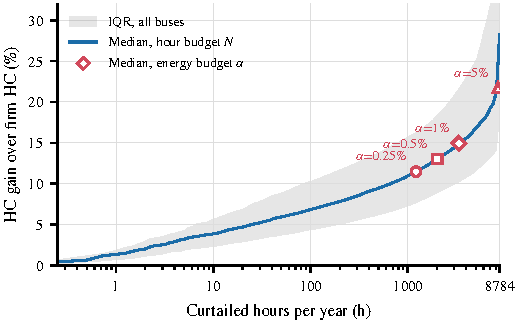
\includegraphics[width=\columnwidth]{figs/fig_duration.pdf}
\caption{HC gain over firm HC versus curtailed hours per year (logarithmic axis), all \nBus~buses, OLTC base case. The line is the hour-budget HC; markers are the medians of energy-budget HC and of its curtailed hours.}
\label{fig:hours}
\end{figure}

\begin{table}[t]
\centering
\caption{Firm HC and Median Flexibility Gains by Grid}
\label{tab:res}
\setlength{\tabcolsep}{2.5pt}
\begin{tabular}{lccccccc}
\toprule
 & Firm HC & \multicolumn{3}{c}{Gain, energy budget (\%)} & Gain & \multicolumn{2}{c}{At $\alpha=1\%$} \\
\cmidrule(lr){3-5}\cmidrule(lr){7-8}
Grid & median & 0.25\% & 0.5\% & 1\% & 100 h & Hours & Longest \\
 & (MW) & & & & (\%) & (h/yr) & event (h) \\
\midrule
Rural & 5.62 & 9.8 & 11.4 & 13.3 & 5.4 & 3072 & 19.0 \\
Semi-urban & 6.18 & 11.0 & 12.4 & 14.2 & 6.7 & 3518 & 20.8 \\
Urban & 5.77 & 11.6 & 13.2 & 15.1 & 7.0 & 3472 & 18.5 \\
Commercial & 7.22 & 13.1 & 14.7 & 16.8 & 8.5 & 2945 & 18.8 \\
\bottomrule
\end{tabular}
\vspace{2pt}
\begin{minipage}{\columnwidth}\footnotesize  Gains are medians over buses of $H_k/H_k^{\mathrm{firm}}-1$. The 100~h column allows curtailment in at most 100 hours per year.\end{minipage}
\end{table}

\begin{table}[t]
\centering
\caption{Contract Parameters Implied by Each Budget (Pooled Medians, Perfect Foresight)}
\label{tab:contract}
\setlength{\tabcolsep}{3pt}
\begin{tabular}{lcccc}
\toprule
 & \multicolumn{3}{c}{N-0} & N-1 \\
\cmidrule(lr){2-4}\cmidrule(lr){5-5}
Parameter & $\alpha=0.25\%$ & $\alpha=1\%$ & 100 h & $\alpha=1\%$ \\
\midrule
Firm HC (MW) & 6.13 & 6.13 & 6.13 & 2.88 \\
Added capacity (MW) & 0.62 & 0.82 & 0.34 & 1.32 \\
Gain over firm HC (\%) & 11.5 & 15.0 & 6.8 & 50.3 \\
Curtailed hours (h/yr) & 1213 & 3350 & 100 & 1536 \\
Events (per year) & 926 & 1263 & 224 & 1060 \\
Median event length (min) & 30 & 45 & 15 & 30 \\
Longest event (h) & 15.0 & 19.0 & 3.3 & 15.8 \\
Deepest curtailment (\% of $P$) & 10 & 13 & 6 & 33 \\
Curtailed energy (\%) & 0.25 & 1.00 & 0.01 & 1.00 \\
\bottomrule
\end{tabular}
\vspace{2pt}
\begin{minipage}{\columnwidth}\footnotesize Medians over buses of each statistic, so they need not multiply. N-1: planning band after outages. All values assume the headroom is known in each 15-min interval (forecasts: Section~\ref{sec:sens}).\end{minipage}
\end{table}


For a connecting customer at the median bus, a 1\% budget adds \robPerfaddMW~MW (95\% interval \ciAddLo--\ciAddHi~MW) to a firm HC of \firmPoolMed~MW. In exchange the load is curtailed in \poolGchrs~h/yr (\hrsOneShare\% of the year), in about \poolGcnev~events with a median length of \poolGcmedevmin~min, with a median deepest curtailment of \depOne\% of nameplate, while losing 1\% of its energy. Whether this is worth it depends on the customer's cost of interruption and the reinforcement cost and delay avoided; no cost model is included.

At the connection point, the 85~h/yr of the bulk-system study \cite{duke} buys only \gEightyFive\%, and network and system curtailment hours need not coincide. Gu \emph{et al.} reported a 78\% gain for 1\% of intervals curtailed in their copperplate example \cite{gu2026hicss}; the same budget gives a median of \gonepctint\% here. Applying their setup (copperplate, transformer 10\% above the peak load, no DG) to our profiles gives \cpLo--\cpHi\%, so the difference stems from how much spare capacity the network has, not from the load data.

\subsection{Variation Between Buses}
With OLTC (Fig.~\ref{fig:binding}), median gains are similar at the \nVlow~undervoltage-limited buses (\gVlow\%) and the \nLine~line-limited buses (\gLine\%); with fixed taps, voltage-limited buses gain far more (\sensFixgv\% versus \sensFixgl\%), so that difference reflects the voltage-control assumption. Simple indicators are poor predictors: the rank correlation of the gain with the Th\'evenin (driving-point) impedance at the bus is \spZth~and with firm HC \spFirm.

\begin{figure}[t]
\centering
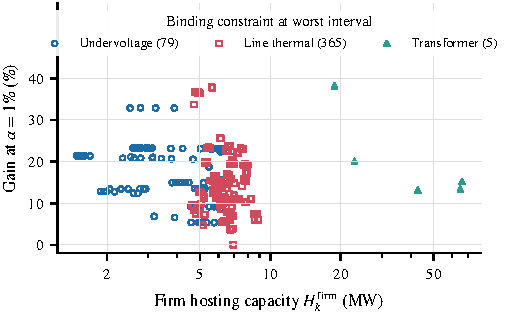
\includegraphics[width=0.92\columnwidth]{figs/fig_binding.pdf}
\caption{HC gain at $\alpha=1\%$ versus firm HC; one marker per bus, by the constraint binding at its worst interval (OLTC base case).}
\label{fig:binding}
\end{figure}

\subsection{Robustness}\label{sec:sens}
\emph{Network assumptions} (Table~\ref{tab:sens}). A load with a daily swing of $\pm$20\% (Table~\ref{tab:sens}) gains \shpRowGone\% at 1\% with fewer curtailed hours. SimBench scenario 2 (future load, DG, and storage) gives \sensStwogO\%. At unity power factor (\pfN~buses) the gain changes from \pfGainA\% to \pfGainB\%.

\emph{N-1 line outages.} Each of the \nmoN~in-service line outages is followed by closing the normally open tie that restores all disconnected buses (the one with the largest worst-case margin if several can; \nmoUnr~spur outages leave their buses unsupplied), with the base-case limits. The headroom is the minimum over the intact network and all outages, i.e., the new load is curtailed preventively whenever an outage would cause a violation. Median firm HC falls from \sensBasefirm~to \sensNmofirm~MW, and undervoltage limits \sensNmonv~buses instead of \sensBasenv. Because the post-outage headroom varies more, the 1\% gain rises to \sensNmogO\% (\sensNmowgO\% with the wider band), and \sensNmohOZZ\% for 100~h; at the median bus the 1\% budget adds \ctNadd~MW instead of \ctBadd~MW, with fewer curtailed hours but deeper curtailment (Table~\ref{tab:contract}). Capping curtailment at \depCap\% of nameplate, as demonstrated for a data center \cite{colangelo2025}, leaves the N-0 gain unchanged (\depNZshare\% of buses capped) but limits the N-1 gain to \depNOgain\% (\depNOshare\% of buses capped). Flexibility is thus worth more where the operator plans for N-1; corrective curtailment, applied only after an outage, is bounded by the intact network: at the median bus it raises the 1\% nameplate from \corPreMW~MW to at most \corCorMW~MW, but the load must then shed \corDepth\% of it after the worst outage, within the restoration time. Outage rates are not modeled. Halving the non-urban transformer limits for N-1 would bind at about one busbar bus per grid.

\begin{table}[t]
\centering
\caption{Sensitivity to Network Assumptions (Pooled Medians, All Buses)}
\label{tab:sens}
\setlength{\tabcolsep}{2.4pt}
\begin{tabular}{lcccccc}
\toprule
Configuration & Firm & \multicolumn{2}{c}{Gain (\%)} & Gain & Hours & Buses \\
\cmidrule(lr){3-4}
 & (MW) & 0.25\% & 1\% & 100 h (\%) & at 1\% & V/L/T \\
\midrule
Base (ideal OLTC) & 6.13 & 11.5 & 15.0 & 6.8 & 3350 & 79/365/5 \\
Fixed taps & 5.89 & 13.2 & 16.7 & 8.2 & 3190 & 106/341/2 \\
N-1, planning band & 2.88 & 38.7 & 50.3 & 29.4 & 1536 & 241/203/5 \\
N-1, 0.90--1.10 p.u. & 3.60 & 29.2 & 38.8 & 20.2 & 1781 & 116/328/5 \\
Scenario 2 (future) & 5.92 & 14.1 & 18.8 & 8.1 & 2493 & 82/373/5 \\
\bottomrule
\end{tabular}
\vspace{2pt}
\begin{minipage}{\columnwidth}\footnotesize V/L/T: buses whose firm HC is set by undervoltage, line, or transformer limits; one scenario-2 bus next to a pre-existing overvoltage is counted by the limit violated just above its headroom.\end{minipage}
\end{table}


\emph{Imperfect foresight} ($\alpha=1\%$, alternating weeks). Persistence of the measured headroom was the best 15-min forecast, with a median gain of \fcPFifteengain\% (seasonally adjusted persistence \fcSAFifteengain\%, net-load forecast \fcNLFifteengain\%). Day-ahead forecasts kept \fcRangeDagainLo--\fcRangeDagainHi\%, the net-load forecast doing best, about half the 15-min gain. Of the test cases, \fcRangeFifteenviolLo--\fcRangeFifteenviolHi\% (15-min) and \fcRangeDaviolLo--\fcRangeDaviolHi\% (day-ahead) had a violation, typically in \fcVintLo--\fcVintHi~intervals by \fcExcLo--\fcExcHi\% of nameplate. Training on the first half of the year and testing on the second, and the reverse, gave similar results (\fcBlkFifteengainLo--\fcBlkFifteengainHi\% and \fcBlkFifteenviolLo--\fcBlkFifteenviolHi\% for 15-min, \fcBlkDagainLo--\fcBlkDagainHi\% and \fcBlkDaviolLo--\fcBlkDaviolHi\% day-ahead), so alternating weeks do not materially flatter the forecasts. Margins therefore need a reserve beyond what one year of data shows.

\emph{Static baseline.} Holding the load at firm HC in a fixed window $W$ and at $P=\min_{t\notin W}\bar P_k(t)$ otherwise, without measurement, gains a median of \todWingain\% with November--February as $W$ (energy loss \todWinen\%) and \todEvegain\% with 16:00--22:00 daily; chosen on the first half-year, it violated limits in the second at \todWinvOT\% of buses (\todWinvTO\% the other way round). Real-time curtailment is what delivers the gain.

\section{Discussion and Conclusion}
The answer depends on the planning standard. With all lines in service, flexibility is a moderate lever in these grids (\poolGcmed\% at 1\%), because spare capacity is large relative to load variability; where the operator plans for N-1 and curtails preventively, it adds \sensNmogO\% (\ctNadd~MW at the median bus), because post-outage headroom varies far more; curtailing only after outages allows more but requires shedding about half the load quickly. In every case its cost is measured in hours and response capability more than in energy. Flexible connection agreements for MV loads should therefore state the parameters in Table~\ref{tab:contract} (hours, events, duration, depth, response time), not an energy budget alone. Most of the value requires near-real-time headroom estimation and response; with day-ahead notice, as in hour-limited products \cite{tennet_tdtr}, none of the forecasts tested here kept more than \fcDaMaxAll\%.

Results will differ with topology, thermal ratings, voltage control, and reverse power flow. Absolute HC depends on the synthetic one-year profiles, the ideal OLTC, DG without voltage control, and, for N-1, the preventive criterion and post-outage voltage band. Each result assumes a single new connection, so it bounds what a first applicant can obtain; 15-min averaging hides faster variation, so event counts are lower bounds. Load shifting (energy recovered later, analyzed in \cite{gu2026hicss}) and costs are not modeled.

\section*{Acknowledgment}
In accordance with IEEE policy on AI-generated content, the author discloses that Claude (Opus 5.5, Anthropic) was used extensively in preparing this paper. The author initiated and directed the project, selected the venue, decided to add the load-shape analysis, and reviewed the method, the results, and the text. Claude wrote the simulation, analysis, and plotting code; ran the simulations; produced all figures and tables; carried out the literature search and reference checking; and drafted the text of all sections. The author takes responsibility for the content.


\bibliographystyle{IEEEtran}
\bibliography{refs}

\end{document}
